\documentclass[12pt,a4paper]{article}
\usepackage[utf8]{inputenc}
\usepackage[T1]{fontenc}
\usepackage[spanish]{babel}
\usepackage{amsmath}
\usepackage{amsfonts}
\usepackage{amssymb}
\usepackage{graphicx}
\usepackage[left=3.00cm, right=3.00cm, top=2.50cm, bottom=2.50cm]{geometry}
\author{Caamiña Quineros, Daniela Beatriz\\ \and Yapura, Cristian Alejandro}
\title{Proyecto final}
\newcommand{\grad}{$^{\circ}$}
\begin{document}
	\maketitle
	\newpage
	\thanks{Agradecimiento}
	\newpage
	\tableofcontents
	\newpage
	\listoffigures
	\newpage
	\section{Introducción}
	\section{Objetivo}
	\section{Palabras claves}
	\newpage
	\part{Marco teórico}
	\section{Túnel del viento}
	\subsection{¿Qué es?}
	\subsection{Clasificación}
	\subsection{Historia del Túnel UNPSJB}
	\cite{TunelUNPSJB} El túnel aerodinámico del Laboratorio de Mecánica de Fluidos (LMF) de la Facultad de Ingeniería de la Universidad Nacional de la Patagonia San Juan Bosco (UNPSJB) es un circuito abierto (tipo Eiffel) con cámara de ensayos cerrada. Puede clasificarse como un túnel “pequeño de baja velocidad”, con una longitud total de 11m, una velocidad máxima de 18 m/s y una cámara de ensayos con un área de 0,8m2.
	\\
	La entrada del túnel cuenta con canalizadores, comúnmente denominados "panal de abejas", que favorecen la formación de un flujo uniforme y homogéneo propiciando mejores resultados en los experimentos.
	\\
	La cámara de ensayos es vidriada para poder observar con claridad el flujo y está incorporada en un módulo extraíble del túnel, lo cual permite fácil acceso para el armado de los distintos objetos a ensayar.
	\\
	La variación de la velocidad del aire dentro de la cámara se consigue por dos vías: modificando la velocidad del motor para lograr una aproximación, y mediante la apertura de compuertas ubicadas entre el rodete y la zona de ensayo, para el ajuste fino. La toma aire desde el exterior a través de las compuertas actúa como by-pass, modificando el flujo principal del túnel y controlando su velocidad.
	\\
	Los distintos ensayos que se realizan en el túnel son:
	\\
	- Determinación de coeficientes de resistencia y sustentación de distintos cuerpos y perfiles aerodinámicos.
	- Determinación de distribución de presiones a través de diferentes objetos como perfiles aerodinámicos, edificios, puentes, automóviles, etc.
	- Visualización con humo del flujo a través de distintos obstáculos.
	- Estudio del comportamiento dinámico de generadores eólicos.
	- Calibración de anemómetros. 
	\section{Cálculo de la densidad del aire}
	\section{Variador de velocidad}
	\subsection{¿Qué es y para que se utiliza?}
	\subsection{Variador ----- modelo que tenemos}
	\section{Comunicación I2C}
	\newpage
	\part{Desarrollo}
	\section{Primeras pruebas}
	\subsection{Electrónica- Placas}
	\subsubsection{SHT31-SHT21}
	SHT31 es un sensor digital de temperatura y humedad relativa. Posee protocolo I2C.
	\paragraph*{Especificaciones}
	\begin{itemize}
		\item   Voltaje de operación: 2.4 V a 5.5 V.
		\item	Rango de temperatura: -40\grad C a 12\grad C.
		\item   Resolución de temperatura: 0.015\grad C
		\item	Precisión de temperatura: 0.2\grad C 
		\item	Rango de humedad: 0 a 100\% RH
		\item   Resolución HR: 0.01 \% RH
		\item   Precisión HR: 2\% RH
		\item Frecuencia de muestreo: 157 Hz.
	\end{itemize}
		\begin{figure}[htb]
	\centering
	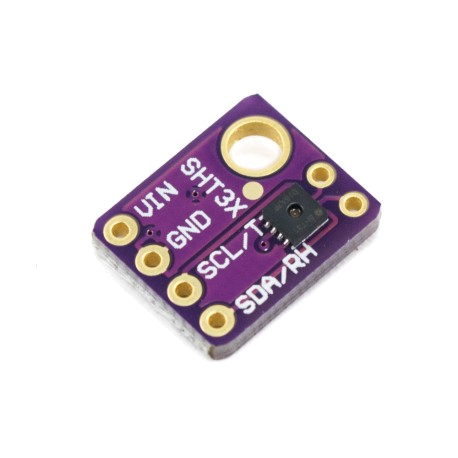
\includegraphics[scale=0.35]{SHT31.png}
	\caption{Placa SHT31}
	\label{fig:SHT31}
		\end{figure}
	
	\subsubsection{BME280}
	BME280 es un dispositivo que mide presión atmosférica, temperatura y humedad relativa, con gran precisión, bajo consumo y compacto. Utiliza protocolo I2C para su comunicación.
		\paragraph*{Especificaciones}
		\begin{itemize}
		\item   Voltaje de operación: 1.8 V a 3.3 V.
		\item	Rango de temperatura: -40\grad C a 85\grad C.
		\item   Resolución de temperatura: 0.01\grad C
		\item	Precisión de temperatura: 1\grad C 
		\item	Rango de humedad: 0 a 100\% RH
		\item   Precisión HR: 3\% RH
		\item Rango de Presión: 300 a 1100 hPa (0.3-1.1bar)
		\item Resolución de presión: 0.16 Pa
	\end{itemize}
	
		\begin{figure}[htb]
		\centering
		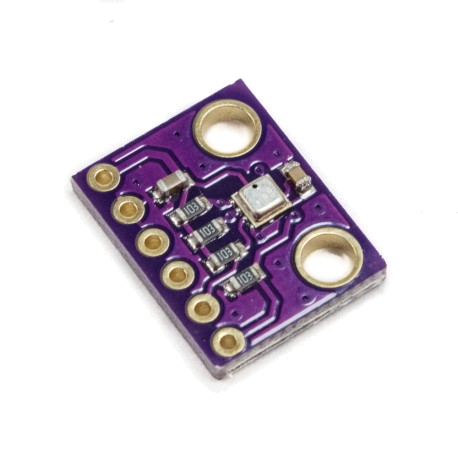
\includegraphics[scale=0.35]{bme280.png}
		\caption{Placa BME280}
		\label{fig:BME280}
		\end{figure}
	
	\subsubsection{MPX7002}
	
	\subsection{Matlab}
	\subsection{Arduino}
	\section{Lazo de control}
	\subsection{Comunicación del variador de Velocidad}
	\subsubsection{0-10V}
	\subsubsection{4-20mA}
	\subsubsection{MODBUS}
	\section{Microcontrolador}
	\subsection{Arduino- CIAA}

\newpage
\bibliography{biblio}
https://mauricioanderson.com/curso-latex-referencias-bibliografia-bibtex/ ver esto
\begin{thebibliography}{0}
	\bibitem{TunelUNPSJB} http://www.ing.unp.edu.ar/mecanica/Paginas/Tunel.htm.
	\bibitem{Luckie2010} Matthew Luckie. CScamper: a scalable, extensible packet 
	prober for active measurement of the internet, 2010.
\end{thebibliography}
\newpage
\part{Anexos}





\end{document}